\documentclass{article}
\usepackage[utf8]{inputenc}
\usepackage{graphicx}
\usepackage{amssymb}
\title{Cognitive Science 1 \\ Midterm 2 Study Guide}
\author{Benjamin Lee \& Aparna Bharathala}
\date{March 2018}

\begin{document}

\maketitle

% \textbf{Key Concepts:}

% \begin{itemize}
%     \item Lecture 9: Categories: Prototypes and Stereotypes
%     \begin{itemize}
%         \item 3 Approaches: Exemplar, Feature, Prototype
%         \item Hierarchy in categorization: Superordinate, Basic-Level, Subordinate
%         \item Graded membership, family resemblance, fuzzy boudnaries
%     \end{itemize}
% \end{itemize}

\section{Lecture 8: Categories and Stereotypes}
What are \textbf{concepts}? 
\begin{itemize}
    \item Concepts are thoughts and can be used to \textbf{build relationships} between thoughts
    \item Concepts are the elements of reason and constitute the \textbf{meaning of words and linguistic expressions}
    \item In short: Mental representations that enable individuals to categorize objects in one way or another.
\end{itemize}
\textbf{Categorization:} the capacity to systematically group events and objects \\

\subsection{3 Approaches to Categorization: Exemplar, Feature, Prototype}

\noindent \textbf{Exemplar (experiences):}
\begin{itemize}
    \item Categorization involves comparing some object or event with previous instances stored in memory 
    \item Example: I categorize some new animal as a dog if it matches with previous instances of dogs I've stored in memory
    \item Similarity to instances already formed: 
        \subitem Based on experience
        \subitem Con: Categories $\rightarrow$ realize something belongs to a category but haven't seen it before
    \item Difficulty: within a category, the entities are very different from each other
\end{itemize}

\noindent \textbf{Feature (Classical View):}
\begin{itemize}
    \item Categorization of objects and events is based on a set of \textbf{necessary and sufficient conditions} for category membership
    \item Example: the category bachelor must be adult, human, male, unmarried, in order to qualify for membership. 
    \item All features must be present (equal membership)
    \item Clear-cut (no fuzzy boundary)
\end{itemize}

\noindent \textbf{Prototype:}
\begin{itemize}
    \item Categorization takes place on the basis of a prototype, a highly salient or typical member of the category (average member)
    \item Example: I categorize an object as a chair depending on the degree to which it looks like a typical chair. Typical dog, house, summer day, etc. 
    \item Some members of a category are more typical than others 
    \item Fuzzy boundary (not clear or exact)
\end{itemize}

\subsection{Graded Membership and Family Resemblance}

\begin{figure}[htp]
\centering
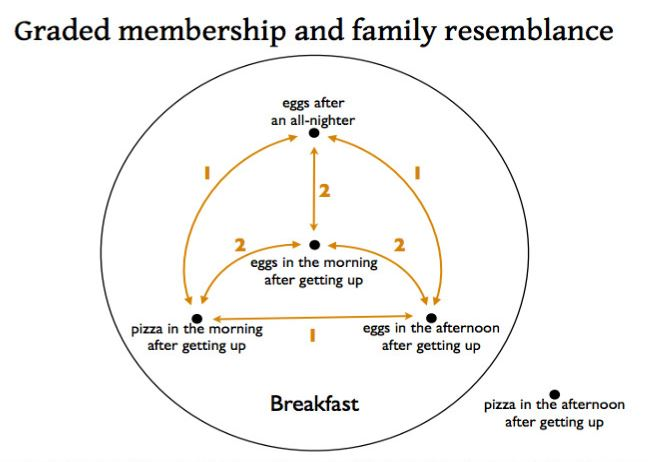
\includegraphics[width=10cm]{images/Breakfast.JPG}
\caption{Graded membership}
\label{fig: Graded Membership}
\end{figure}

\noindent \textbf{Graded membership:} Some members are better than others, (certain categories are held in a higher regard than others) \\
\textbf{Family resemblance:} things in the category share features with each other. (Example: eggs are related to breakfast, which is what you eat in the morning, after waking up) \\
\textbf{Fuzzy boundaries:} hard to identify the boundary (Example: you can have pizza in the morning and still consider it breakfast.) \\

Prototypical breakfast: 
\begin{itemize}
    \item Eaten early in the day
    \item after a period of sleep 
    \item has a special menu (eggs, toast, etc)
    \item remove any feature and we still have a breakfast of some sort (can't remove 2 or more features or else it won't be breakfast anymore)
\end{itemize}
\textbf{Heuristic search} (not perfectly accurate search but close enough and fast) \\

\noindent Misleading of prototypes: 
\begin{itemize}
    \item Conjunction fallacy
        \subitem It is impossible for the conjuction of two conditions to be more probable than either conjunction alone, but people still fall under the pretense that a category has both these conditions 
\end{itemize}

\begin{figure}[htp]
\centering
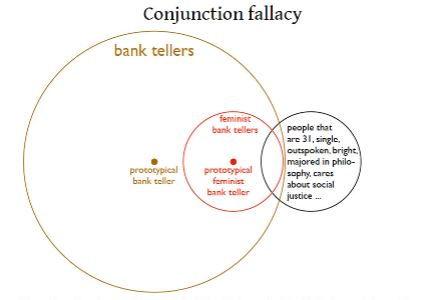
\includegraphics[width=10cm]{images/conjunctionfallacy.JPG}
\caption{Conjunction Fallacy Example}
\label{fig: conjunction}
\end{figure}

\subsection{Hierarchy in Categorization: Superordinate, Basic-level, Subordinate}

\begin{figure}[htp]
\centering
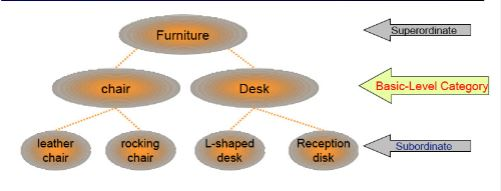
\includegraphics[width=10cm, height=5cm]{images/prototypelevel.JPG}
\caption{Categories and Prototypes: levels}
\label{fig: categories}
\end{figure}

\begin{itemize}
    \item \textbf{Superordinate} (superordinate semantic category)
        \subitem Category at the top from which the others branch out
        \subitem Most general level of a categorization (i.e. Furniture)
    \item \textbf{Basic-Level}
        \subitem more specific category to superordinate (ex. chair or desk) 
    \item \textbf{Subordinate} (semantic category) 
        \subitem specific level usually "type of" (ex leather chair, rocking chair) \\
        
\textbf{Three ways of examining the categories we form: }
    \subitem relations between categories (basic-level category) 
    \subitem internal category structure (radial category) 
    \subitem instances of category members (prototypes) 
\end{itemize}

Categorization has been noted to have some sort of hard-wiring before we are even born. By age 3 or even infancy, children classify the people they meet into groups. \\


\newpage 
\section{Lecture 9: Linguistics: Aphasias, Metaphors}

\textbf{Language is special:}
\begin{enumerate}
    \item Relies on \textbf{mental representations} (trouble for behaviorism) 
    \item Particular strengths and weaknesses: great for things that aren't here
    \item Uniquely \textbf{human}: suggests an innate basis, trouble for empiricism (all knowledge is derived from sense-experiences (John Locke, George Berkeley, David Hume) )
    \item \textbf{Potentially infinite}: can always produce novel sentences
\end{enumerate}

\subsection{B.F. Skinner's Radical Behaviorism}
\begin{itemize}
    \item Worked on classical conditioning 
    \item Dispenses with talk of mental states
    \item Aims to explain behaviour in terms of the environment
    \item "recognizes \textbf{no dividing line} between man and brute"
\end{itemize}
 
stimulus $\rightarrow$ \framebox{organisms mental state} $\rightarrow$ response

\subsection{Broca's Area \& Wenicke's Area; corresponding aphasias}
 
\textbf{Aphasia:} "without/lacking speech" \\
 
\noindent \textbf{Broca's Area:}
\begin{itemize}
    \item Involved in speech production (ability to produce spoken language) 
    \item Located in left frontal hemisphere
    \item \textbf{Broca's Aphasia:} damage to Broca's area results in the loss of speech production
\end{itemize}
 
\noindent \textbf{Wernicke's Area:}
\begin{itemize}
    \item Involved in the comprehension/understanding of spoken language
    \item located in left temporal lobe 
    \item \textbf{Wernike's Aphasia:} damage to Wernicke's area results in loss of language comprehension. May sound fluent in language, but lacks all meaning. 
\end{itemize}

\noindent \textbf{Kim et al.(1997):} Used fMRI to investigate multiple languages in brain 
\begin{itemize}
    \item Anatomical separation of the two languages in Broca's area varies depending on the time the second language was acquired. (early childhood or adulthood)
    \item Age may be signnificant inn lannguage functional organization. 
\end{itemize}

\noindent \textbf{Alexia:} the individual cannot read but can still write \\
\textbf{Agraphia:} the individual can reason normally, but cannot write \\
 
\noindent \textbf{Chomsky's Universal Grammar:} proposes a set of rules intended to explain language acquisition in child development \\

\noindent \textbf{Recursion:} 
\begin{itemize}
    \item Sentences are formed from clauses 
    \item The property of a system that permits the embedding of an element of the system within itself 
    \item Essentially, you can continuously create endless sentences with no semantics
    \item Example:
        \subitem This is the house that Jack built.
        \subitem This is the cheese that lay in the house that Jack built.
\end{itemize}

\noindent \textbf{Critical Period:} If linguistic experience is missing in the critical period (early childhood) language ability is impaired. \\
Case Studies: Victor the "wild child" and Genie \\

\noindent \textbf{Mirror Neurons:} Neurons fire when you see action or perform it
\begin{itemize}
    \item Found on accident when researchers were eating a banana in front of a monkey. They left the probe in the monkey and it started firing while the monkey watched them eat a banana. 
    \item Firing thought to be implicated in imitation (crucial ability for learning) 
    \item When areas inn which mirror neurons are located are anatomically connected, they form a mirror neuron system (MNS)
\end{itemize}

\textbf{George Lakoff's Brain Conncept Article:} proposes that the sensory-motor system has the right kind of structure to characterize both sensory-motor and more abstract concepts. \\

\textbf{Key Figures:}
\begin{itemize}
    \item \textbf{Noam Chomsky}
        \subitem View: Humans have innate "language faculty" and that the universal principles of human language reflect intrinsic properties of this language faculty
        \subitem Language is autonomous and separate from concepts
        \subitem Since we can create sentences that have no meaning recursively and endlessly, we can separate syntax and semantics
    \item \textbf{George Lakoff}
        \subitem Aims to link language to everyday thinking. Language recruits perceptual and cognitive processes, and is grounded in our everyday embodied experience. 
        \subitem Meaning is conceptualization (ex: same image can have multiple meanings)
        \subitem Since language derives from meaning, (as in language has to have some meaning because without meaning why would there be language) then we cannot separate syntax and semantics. 
\end{itemize}

\newpage
\section{Lecture 10: Cognitive Linguistics with Teenie Matlock}

\textbf{General goal of Cognitive Linguistics:} Sought deeper explanations and wanted to link language to everyday thinking, link between language and cognition \\
\indent -Focus on semantics mostly\\
\indent -Meaning is dynamic, deep, and bound in our experience \\

\textbf{Spatial metaphors:} those metaphors that have space as their source domain and map the image-schematic structure of space onto that of nonspatial and typically abstract target domains, thus enabling the user to talk about and perhaps even to think of those nonspatial domains in spatial terms. \\

\subsection{Metaphors of motion (Fictive Motion)}
\textbf{Fictive Motion:} the metaphorical motion of an object or abstraction through space. \\

\noindent \textbf{Motion Language: Difference between Actual and Fictive motion}

\begin{enumerate}
    \item \textbf{Actual Motion:} The \textbf{bus} \textit{goes} through town.
        \subitem spatial scene, path, explicit mover, state change
    \item \textbf{Fictive Motion:} The \textbf{road} \textit{goes} through town. 
        \subitem spatial scene, path, no explicit mover, no state change
\end{enumerate}

\noindent \textbf{Types of Fictive Motion:} 
\begin{itemize}
    \item \textbf{Type 1:} TR(Path) associated w/ motion 
        \subitem Ex: The \textbf{road} runs along the shore. Can actually traverse the road.
    \item \textbf{Type 2:} TR(Path) not associated w/ motion 
        \subitem Ex: The \textbf{cord} runs along the back wall. Or the table runs along the back wall. Can't traverse the cord or table.  
\end{itemize}
TR(Path): Trajectory of object \\

\noindent Motion language is \textbf{pervasive},  everywhere in language. \\
Conceptualizers "moves" or "scans" the TR(path or linear object) \\
Helps listener/reader compute information about the layout of the scene, especially position of TR relative to LM(landmark). \\

\noindent \textbf{Linguistic Theories of how fictive motion is processed}
\begin{itemize}
    \item \textbf{Dynamic Model:} TR = dynamic representation
        \subitem TR is scanned, built up over time. 
        \subitem Processing depends on context
        \subitem Ex: The road goes from X to Y. (Imagine the road being built up from X to Y)
    \item \textbf{Static Representation:} TR = static representation
        \subitem TR is a temporal structure. 
        \subitem Always processed the same way
        \subitem Ex: The road goes from X to Y. (Imagine the road static, just a straight line from X to Y)
\end{itemize}

\subsection{Aspect}
\textbf{Aspect:} action being done or doing (not just tense as in past tense) 
\begin{itemize}
    \item Influences our attitudes and actions through simulation
    \item Gives info about how events unfold in time, including onset, duration, and completion
    \item Exists in all languages, but grammatically marked in some. 
\end{itemize} 

\noindent \textbf{Imperfective vs. Perfective:}
\begin{itemize}
    \item \textbf{Imperfective:} Past Progressive (PP)
        \subitem Tom \textbf{was hiking} yesterday
        \subitem past tense + VERB\textbf{ING}
    \item \textbf{Perfective:} Simple Past (SP)
        \subitem Tom \textbf{hiked} yesterday.
        \subitem VERB\textbf{ED}
\end{itemize}

\noindent \textbf{Framing:} 
\begin{itemize}
    \item Metaphor is powerful in framing issues, including \textbf{political issues}/campaign messages
    \item metaphors play a big role. Motion metaphors $\rightarrow$ one facet
    \item influence our beliefs
    \item Ex: Obama's campaign slogan, FORWARD vs Romney's campaign slogan, Romney Plan 
\end{itemize}

\newpage
\noindent \textbf{Experiments with Fictive Motion (FM) and Aspect}
\begin{enumerate}
    \item Experiment(FM): Drawing fictive motion 
        \subitem \textbf{\textbf{Logic:}} If people drew longer paths with FM, it might suggest that they simulate motion or scanning, or that they linearly extend TRs in the presence of fictive motion
        \subitem \textbf{Observation:} Longer path with FM
    \item Experiment(FM): Fast and slow story
        \subitem \textbf{Logic:} If FM includes simulation, we should be able to alter that simulation by having people think about real motion in different ways beforehand
        \subitem \textbf{Observation:} Faster response time with fast story
    \item Experiment(FM): Passive listening and eye tracking
        \subitem \textbf{Logic:} If FM involves simulated motion, we might see scanning eye movements along path when people are listening to FM - descriptions and viewing paths
        \subitem \textbf{Observation:} Longer time fixating in the TR region
    \item Experiment(Aspect): PP vs SP (1. was driving/drove, 2. was painting/painted, 3. was planting/planted.) 
        \subitem \textbf{Goal:} Understand how aspect influences the understanding of events, including how we make inferences about actions
        \subitem \textbf{Observation:} More action conceptualized with PP
    \item Experiment(Aspect): blank visual world task
        \subitem \textbf{Goal:} Provide additional evidence and precise measurement of PP associated with more action conceptualization
        \subitem \textbf{Observation:} Past progressive led to many short, distributed fixations
    \item Experiment(Aspect): 2 descriptions about a candidate
        \subitem \textbf{Goal:} Understand how aspect in political messages influence how people think about candidates, including electability. 
        \subitem \textbf{Observation:} PP enhanced attitudes about candidates and electability in some situations, depending on valence, type of event and so on. 
    \item Experiment(Aspect): watch and describe car accidents
        \subitem \textbf{Goal:} Understand effect of aspectual framing of events and leading questions
        \subitem \textbf{Observation:} More action with the PP even though people produced about same number of words and gestures overall. 
\end{enumerate}

\subsection{Sapir-Whorf Hypothesis:}
\begin{itemize}
    \item AKA linguistic relativity hypothesis
    \item Holds that the distinctions within a particular domain expressed in a given language will not be the same as those in any other language
    
    \item \textbf{Strong View:} The structure of your language confines the framework that you are thinking in. 
    \item \textbf{Weak View:} Language is only influencing how you think about things, it doesn't determine what you think
    
    \item Research study on the use of color within those languages (went against hypothesis) 
        \subitem Human beings perceive 11 basic color categories
        \subitem If there are fewer than 11 basic color categories encoded in a language there are strict limitations on which that may be. 
        \subitem Therefore, certain color categories are universally present in human beings
\end{itemize}

\newpage
\section{Lecture 11: Natural Language Processing (Yiyi Chen)}

\textbf{Natural Language Processing (NLP):} Processing language with computers (interdisciplinary: linguistics, computer science and social science) \\

\noindent \textbf{Language Central to Intelligence:} \\
    -Communicating ideas, Represent complex, imperfectly-defined concepts, perform logical reasoning \\

\noindent \textbf{Challenges of NLP:} Language is ...
\begin{itemize}
    \item \textbf{Ambiguous}
        \subitem bank could mean financial institution or the land on the side of a river
    \item \textbf{Flexible}
        \subitem \underline{Nonstandard} English\\
        ur $\rightarrow$ your, U $\rightarrow$ you, 2 $\rightarrow$ to
        \subitem \underline{Idioms} \\
        Bite the bullet/ break a leg
        \subitem \underline{Neologism} \\
        Newly coined word or expression \\
        Bromance, retweet, google, memes
        \subitem \underline{Domain/time/geographical variation} \\
        Though this be madnesss, yet there is method in't
    \item \textbf{Context dependent}
\end{itemize}


\noindent \textbf{Representation of Language:} 
\begin{itemize}
    \item Word: Basic element of speech or writing
        \subitem Red tape \textbf{holds up} new bridges
    \item Syntax: Arrangement of words (structural)
        \subitem The boy saw the bear \textbf{with the telescope}
    \item Semantics: Meanings and relations of words (functional)
        \subitem Teacher \textbf{strikes idle} kids
    \item Discourse: Linguistic expression beyond the boundary of the sentence
        \subitem The \textbf{first one}
\end{itemize}
 
\subsection{Methods}
\begin{itemize}
    \item \textbf{Rule Based Systems:} 
        \subitem Basic Idea: If... then... statements
        \subitem Tokenization: task of breaking down a sentence into tokens (words) 
        \subitem Stemming: task of trimming a word into its root form (sleeping, sleepy, sleeps, sleep)
    \item \textbf{Probabilistic Models}
        \subitem Basic Idea: You are more likely to say "I went to sleep last night" than "I went to class last night"
        \subitem Applications: Naive Bayes, logistic regression, HMM, MEMM, CRF, language models 
        \subitem Part of speech tagging, machine translation, spam detection
    \item \textbf{Neural Networks}
        \subitem Basic Idea: Collective workings of the neurons 
\end{itemize}
\textbf{Rule Based} $\rightarrow$ \textbf{Probabilistic Methods} $\rightarrow$ \textbf{Neural Networks} (requires more data as you move left to right)\\
\textbf{Neural Networks}  $\rightarrow$ \textbf{Probabilistic Methods} $\rightarrow$ \textbf{Rule Base} (requires more explictness in domain knowledge embedding as you move left to right)

\subsection{Word2Vec (Shallow Neural Network Algortihm)}
Vector representation of word with semantic implication. \\
Male-Female: Man $\rightarrow$ Woman \& King $\rightarrow$ Queen \\
Verb Tense: Walking $\rightarrow$ Walked \& Swimming $\rightarrow$ Swam \\

\noindent Can numerically represent words with Word2Vec \\
Ex: (WATER - WET) + FIRE = FLAMES \\
(PARIS - FRANCE) + ITALY = ROME \\

Generative vs Cognitive Linguistics

\newpage 
\section{Lecture 12: Neural Networks, Connectionism, A.I.}

A.I.: The science of making machines that \textbf{think and act} like humans, think and act \textbf{rationally} \\

\subsection{What Can A.I. Do?}
\begin{itemize}
    \item \checkmark Play a decent game of table tennis? 
    \item \checkmark Drive safely along a curving mountain road?
    \item \checkmark Drive safely on University Avenue?
    \item \checkmark Buy a week's worth of groceries on the web?
    \item $\boxtimes$ Buy a week's worth of groceries at Trader Joes? 
    \item ? Discover and prove a new mathematical problem? 
    \item $\boxtimes$ Converse successfully with a person for an hour?
    \item $\boxtimes$ or ? Perform a complex surgical operation? (depends)
    \item \checkmark Unload a dishwasher and put all the dishes away?
    \item \checkmark Translate spoken Chinese into English real time?
    \item $\boxtimes$ Write an intentionally funny story?
\end{itemize}

\subsection{Alan Turing and the Turing Test}

\begin{itemize}
    \item Turing machine helped computer scientists understand the limits of mechanical computation
    \item Explored how to \textbf{judge success} in making \textbf{intelligent} machines.
\end{itemize}

\noindent \textbf{Turing Test:} Test of a machines ability to exhibit intelligent behavior equivalent to or indistinguishable from that of a humans. \\

\noindent \textbf{Problems with Turing Test}
\begin{itemize}
    \item Machines lacking consciousness
    \item Missing human attributes: creativity, making mistakes, learning, etc. 
    \item Can we really conclude intelligence if it does pass?
\end{itemize}

\subsection{Strong vs Weak A.I.}
\textbf{Weak(model of mind):} We can develop artificial systems that act intelligently \\
\indent -Most AI aims at intelligent action \\
\indent -Turing test will be passed by Weak AI \\
\noindent \textbf{Strong(actual mind):} Artificial systems that really think. \\

\subsection{Chinese Room Argument}
If a machine can convincingly simulate an intelligent conversation, does it necessarily understand? \\
\textbf{Searle Argument:} "The point is this: if the man in the room does not understand Chinese on the basis of implementing the appropriate program for understanding Chinese then neither does any other digital computer solely on that basis because no computer, qua computer, has anything the man does not have." \\
\textbf{Shortened:} Just as the man can translate Chinese to English, so can a machine, but in terms of understanding, the man doesn't, so how can a machine understand. \\
The ability to process Chinese [syntax] does not equate understanding of Chinese [semantics] \\
Syntax $\neq$ Semantics \\
Acting intelligently $\neq$ Thinking intelligently \\

\noindent\textbf{Systems Reply: } 
\begin{itemize}
    \item Central Idea: \\
There might be understanding by a larger entity = here, the whole system. While the man running the program does not understand Chinese, the man is just part (CPU) of a larger system which includes instructions, memory, etc 
    \item 
Searle's response: \\
In principle, the man can internalize the entire system, memorizing all the instructions and the database, and doing all the calculations in his head. He could then leave the room and wander outdoors, perhaps even conversing in Chinese. But he still would have no way to attach "any meaning to the formal symbols"
\end{itemize}

\noindent\textbf{Robot Reply:} 
\begin{itemize}
    \item Central Idea: \\
A variation on the system could make it understand - here, the computer may understand if we embed it in a robotic body, which interacts with the physical world via sensors and motors. This way, it could learn by seeing and doing, by having experiences beyond the room. It could come to attach meanings to symbols and actually understand naturally language.  
    \item 
Searle's response: \\
All the sensors do is provide additional input to the computer - and it will be just a syntactic input 
\end{itemize}


\noindent\textbf{Brain Simulator Reply:} 
\begin{itemize}
    \item Central Idea: \\
A variation on the system could make it understand - here, the computer may understand if it simulated the operation of a human brain. The program would simulate the actual sequence of nerve firings that occur in the brain of a native Chinese language speaker when that person understands Chinese - every nerve, every firing. 
    \item Searle's Response: \\ 
it's as if the man has a huge set of valves and water pipes, in the same arrangement as the neurons in a native Chinese speaker's brain. The program now tells the man which valves to open in response to input. It is obvious that there would be no understanding of Chinese. 
\end{itemize}

\subsection{McCulloch-Pitts Neuron (Machine Neuron)}
\begin{figure}[htp]
\centering
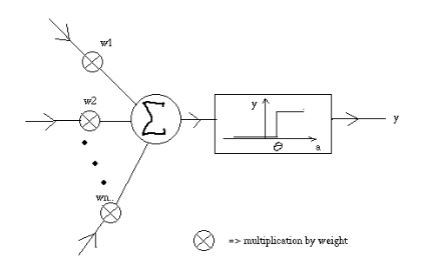
\includegraphics[width=8cm]{images/mccullochneuron.JPG}
\caption{McCulloch Neuron}
\label{fig: Machine neuron}
\end{figure}

\begin{figure}[htp]
\centering
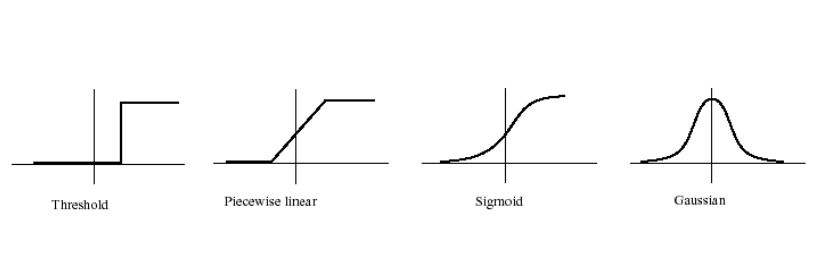
\includegraphics[width=15cm, height=6cm]{images/activationfunctions.JPG}
\caption{Activation Functions}
\label{fig: Act func}
\end{figure}

\textbf{Relation of Hebbian Learning and Artificial Neural Networks:} \\
Hebbian Learning or Associative Learning: Useful neural connections get strengthened over time, and not so useful ones die out. When neurons fire together, they wire together. \\
ANN Works similarly, where the system learns the irght weights (signifying the importance of a feature from the training data through \textbf{back propagation}. With training the weights of useful features in the network get strengthened (increase in value), and those of not so useful ones get weakened (decrease in value). This learning process is similar to Hebbian learning in the sense that the weights are determined though iterations of learning and reinforcement/punishment. \\

\textbf{Examples of Artificial Neural Network:} 
\begin{figure}[h]
\centering
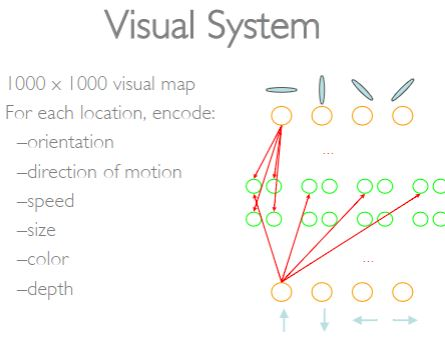
\includegraphics[width=6cm]{images/visualsys.JPG}
\caption{Visual System}
\label{fig: vissys}
\end{figure}

\begin{figure}[h]
\centering
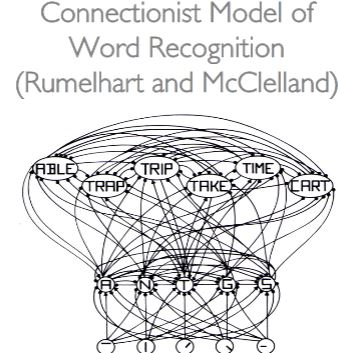
\includegraphics[width=6cm]{images/connectionist.JPG}
\caption{Connectionist Model of Word Recognition}
\label{fig: connectionist}
\end{figure}

\begin{figure}[htb]
\centering
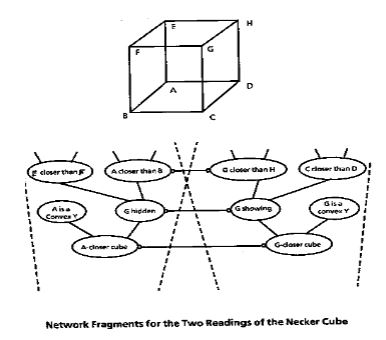
\includegraphics[width=5cm]{images/necker.JPG}
\caption{Necker Cube}
\label{fig: Necker}
\end{figure}


\subsection{Perceptrons}
The simplest kind of "feed forward" neural network. (Originally introduced by Frank Rosenblatt (1985).\\
\textbf{Feed Forward}, refers to the direction in which information/data flows when the neural network is making a prediction, i.e. input layer $\rightarrow$ hidden layer $\rightarrow$ output layer. Features come in from the input layer, the information flows through the network and the system generates some output (some predition/classification result) at the end\\
\textbf{Back Propogation}, refers to the direction in which error/ update flows when the system is learning. During the training stage, we have the data of both the input and desirable output. For a given input, the system compares its prediction with the desirable output, and use  the difference/prediction error to update the network (hebbian learning). This error is therefore fed backward through the system, so the weights in the networks can be adjusted accordingly. The goal is that with these adjustments, the network will learn from its mistakes and give better and better predictions. \\
\textbf{Multilayer Feed Forward Network:} Consists of \textbf{hidden layers} which are these weights that determine the output layer. If the output is not desirable, back propagation is used to adjust the weights in the hidden layer. \\

\begin{figure}[htp]
\centering
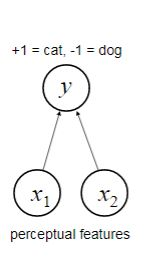
\includegraphics{images/perceptron.JPG}
\caption{Perceptron Simple Feed Forward}
\label{fig: Perceptron}
\end{figure}


\begin{figure}[htp]
\centering
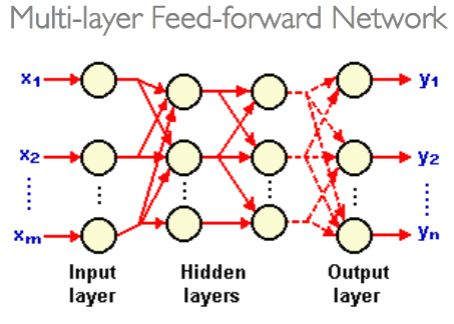
\includegraphics[width=5cm]{images/multilayerfeedforward.JPG}
\caption{Multi-Layer Feed Forward}
\label{fig: MLFF}
\end{figure}

\begin{figure}[htp]
\centering
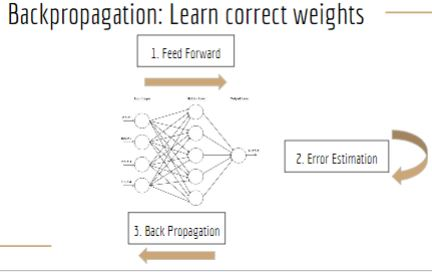
\includegraphics[width=10cm]{images/backprop.JPG}
\caption{Backpropagation}
\label{fig: back prop}
\end{figure}

\newpage
\section{Lecture 13: Guest Lecture Anand Kulkarni on AI}

\textbf{Takeaways:}
\begin{itemize}
    \item What is AI?
        \subitem Study and Engineering of making machines intelligent. Intelligence is broad, but we'll compare it to behaving like a human
        \subitem A.I. is a moving target, we used to think of Chess A.I. as significant, but now we have Google maps and translate and we don't even think of it as A.I. 
    \item Neural Network
        \subitem Model the machine like a brain
        \subitem Brains have neurons, so we make machine neurons, known as Perceptrons
        \subitem Perceptrons are Linear binary classifiers. Linear because we multiply our inputs by weights and then sum them together linearly. (no squared or cubed) And then binary because when we output either a 1 or 0. 
        \subitem Take inputs, multiply by weights and sum them, run through unit step function(activation function). Tells us what the neuron does in response to our input 
    \item Feature sets
        \subitem Build neurons using feature sets (weights). 
        \subitem Features relate to the function we want our A.I. to perform (Ex: We want computer vision, so we need to detect colors, orientation, motion, shape, depth, etc. These are our features)
    \item Deep Learning
        \subitem Multiple-layers in our neural network (i.e. layer is made of multiple perceptrons. Having multiple layers of these perceptrons simulates how neurons send signals to more neurons)
        \subitem Feed Forward Neural Network, goes in one direction. 
    \item AI risks
        \subitem Concerned about bias in our data. 
        \subitem Like a naive human, our A.I. is also naive to something, so we train it with a data sets and back propagation. 
        \subitem However, we want to make sure our data is not biased as well. 
\end{itemize}

\newpage
\section{Lecture 14: "Playing with Perceptrons" (Neha Mittal)}
\textbf{Arthur Samuel} - Father of Machine Learning \\
\indent Created A.I. checker player that beat the checkers champion \\

\noindent \textbf{A.I. Today:} Google search, Facebook Graphs, Amazon Recommendations \\

\subsection{B.F. Skinner's Radical Behaviorism Theory}
Look back to Lecture 9 for definition. \\
\textbf{Machine Learning:} gives computer systems the ability to "learn" with data and not much programming. \\
\textbf{Computer Vision:} Making computers see as humans do. Involves acquiring, processing, analyzing and understanding images and extraction of high dimensional data. \\
\begin{figure}[htp]
\centering
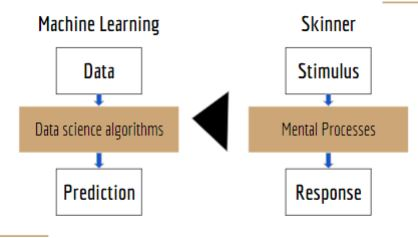
\includegraphics[width=9cm]{images/machinelearning.JPG}
\caption{BF Skinner in relation to Machine Learning}
\label{fig: ML and Skinner}
\end{figure}

\noindent \textbf{Concepts of Machine Learning:} 
\begin{enumerate}
    \item Input(x) and Output(f(x) or y
    \item Classification of Output
    \item Learning aka Training
    \item Training vs Testing Phase
\end{enumerate}

\noindent \textbf{Problems with traditional ML Models:}
\begin{enumerate}
    \item Domain Knowledge
    \item Infinite variations of inputs
\end{enumerate}

\noindent \textbf{Main Concepts of Lecture:}
\begin{itemize}
    \item Featurization
        \subitem These are the weights in our ML neural net. Weighted differently based on importance
    \item Perceptrons: Feed Forward Calculations
        \subitem In the image below, multiply weight by input and sum the weights. 
        \subitem Then we get an activation function which will determine the output. 
    \item Success of deep learning in computer vision: loads of image data made open source \textbf{architecture by hand} instead of feature design by hand
        \subitem \textbf{Feature by Hand:} Focus is ensuring the usefuelness/quality of the features. 
        \subitem \textbf{Architecture by Hand:} Just want to make sure your features are expressive/ contain useful information. Main focus is designing the best architecture that will allow the useful bits in your feature to shine and help you generate the best output.
        \subitem \textbf{Example: predict students grades} \\
        \textbf{Feature by hand:} solve focusing with \textbf{high quality features} that are predictive of students performance, e.g. midterm grades. \\
        \textbf{Architecture by hand:} solve with \textbf{many features} about a student, e.g. midterm scores, breakfast, commute, shoes. 
        \subitem Point is that hopefully the Neural Network will figure out which features are most predictive of the scores drawing from huge data sets. 
        \subitem Example from class: Geoff Hinton and Image Net, Paul Li described as cute
    \item Difference between perceptron and deep learning
        \subitem Perceptron is like the single-layer perceptron earlier in the study guide. It has one hidden layer, which is shallow. 
        \subitem Deep learning is like the Multi-layer feed forward network, where it has multiple hidden layers that take inputs from the previous layer. Deep because of its depth in layers. Look at backpropagation as well. 
\end{itemize}
\begin{figure}[htp]
\centering
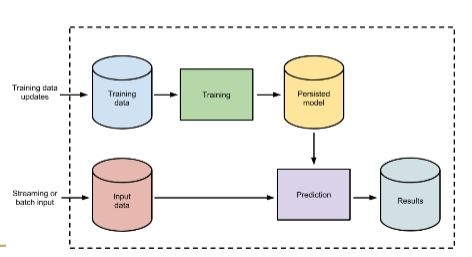
\includegraphics[width=15cm]{images/MLconcept.JPG}
\caption{ML training}
\label{fig: ML}
\end{figure}

\begin{figure}[htp]
\centering
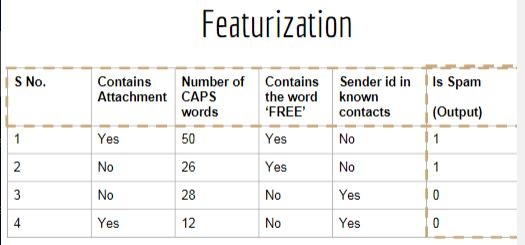
\includegraphics[width=15cm]{images/featurization.JPG}
\caption{Featurization}
\label{fig: featurization}
\end{figure}

\begin{figure}[htp]
\centering
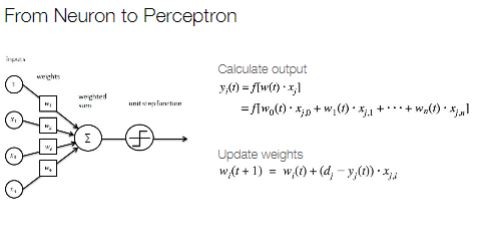
\includegraphics[width=15cm]{images/feedforwardcalc.JPG}
\caption{Perceptron Calculation}
\label{fig: calc}
\end{figure}

\begin{figure}[htp]
\centering
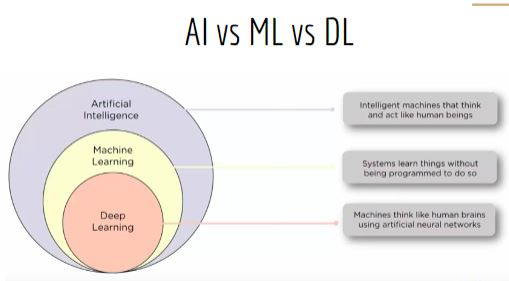
\includegraphics[width=15cm]{images/AIMLDL.JPG}
\caption{AI vs ML vs DL}
\label{fig: aimldl}
\end{figure}

\begin{figure}[htp]
\centering
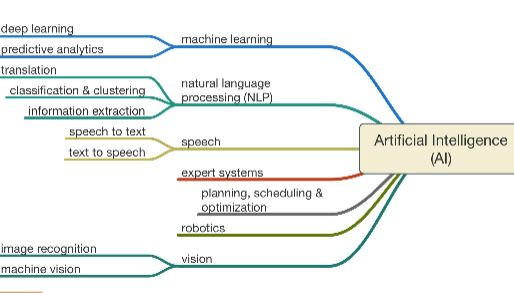
\includegraphics[width=15cm]{images/AI.JPG}
\caption{AI}
\label{fig: ai}
\end{figure}

\end{document}